\chapter{Astrophysical Shocks}

\chapter{Breakdown of Computational Models}

This section contains a breakdown of the cooling and dust models, along with an accompanying flowchart, for the sake of clarity.

\section{Cooling model}

\section{Dust model}

\chapter{Software Carpentry}

\section{Software \& Resource Acknowledgements}

This project relied on a number of resources available from the University of Leeds, as well as many open source projects scattered around the globe.
Not to opine on the importance of open source projects for too long, but we as researchers should be aware of the time, effort and labour of programmers developing open source projects.
Learning that perhaps the bulk of the infrastructure we use rests almost entirely on a series of freely-developed projects came as a shock to me many years ago, and in lieu of payment, this section will acknowledge these projects, to the best of my ability.

This work was undertaken on \texttt{ARC3} and \texttt{ARC4}, part of the High Performance Computing facilities at the University of Leeds, UK.
Much of the earlier development and testing work was undertaken on workstations provided by the department.
In particular was the 44 core workstation my supervisor used\footnote{Which I refer to as \texttt{jumpcannon}, after Annie Jump Cannon, though the name didn't catch on.}, whose computing brunt was used frequently throughout the project.

A good deal of the data reduction of this thesis was conducted using the Python 3 programming language \parencite{10.5555/1593511}, in particular, the following open source modules were used extensively:

\begin{itemize}
  \item \footlink{\texttt{NumPy}}{https://numpy.org/} \parencite{harris2020array}.
  \item \footlink{\texttt{Astropy}}{https://www.astropy.org/} \parencite{astropy:2013,astropy:2018}.
  \item \footlink{\texttt{Matplotlib}}{https://matplotlib.org/} \parencite{Hunter:2007}.
\end{itemize}

\athena{} \parencite{athena} was also used extensively throughout the work in this thesis.
Whilst there are some aspects of this that need further development - in particular, passive scalars in AMR problems - it was found to be extremely robust, and easy to develop for.
Some diagrams in this work, specifically Fig. \ref{fig:quiver-h} and Fig. \ref{fig:quiver-oplus} use the \footlink{Quiver}{https://q.uiver.app/} communicative diagram editor.
GNU Parallel \parencite{tange_2021_5523272} was used to speed up the batch processing of data within this project, if parallel programming is difficult, sometimes the only option is to run many, \textit{many} serial programmes at once.
The \footlink{\texttt{Hyperfine}}{https://github.com/sharkdp/hyperfine} command line benchmarking tool was used to benchmark \athena{} throughout the project, in order to find ideal configuration parameters such as numerical integrators, core counts and meshblock sizes.
Most of the line plots in this project were produced by the 
The \footlink{\texttt{turbo}}{https://ai.googleblog.com/2019/08/turbo-improved-rainbow-colormap-for.html} palette is used for
A modified version of the \texttt{turbo.pal} palette file from the \footlink{\texttt{gnuplotting.org} GitHub repo}{https://github.com/Gnuplotting/gnuplot-palettes/blob/master/turbo.pal} was used to import the colour scheme into \texttt{gnuplot}.

Finally, this thesis was typeset with \LaTeX{}, using the {\TeX}live distribution and \texttt{latexmk} for compilation.
It is abundantly clear that scientists the world over owe an enormous debt of gratitude to Donald Knuth and Leslie Lamport for their work on the \TeX{} and \LaTeX{} projects.
Let's hope that the version $\pi$ update isn't coming too soon.
The thesis template is a modified version of the \footlink{Leeds Condensed Matter Physics Group \LaTeX{} template}{https://github.com/stonerlab/Thesis-template}, which suited the needs of this thesis extremely well.

\section{Parallelism \& Amdahl's Law}
\label{app:parallelism}

% Single threaded 
One of the more prominent mistaken expectations of computing in the last few decades was the idea of extreme scaling of processors.
Early in the lifecycle of the NetBurst architecture, Intel predicted the Pentium 4 and the subsequent generations of processor would scale up to \SI{10}{\giga\hertz}.
This of course, never panned out, only a handful of processors can reliably scale to \SI{5}{\giga\hertz} at a comparatively large thermal penalty, with contemporary high-end desktop processors drawing as much as twice the power of the hottest running NetBurst designs.
Instead, processors, while significantly faster in single threaded applications, have more than one processing core.
In most cases in scientific computing, single-threaded performance has been entirely supplanted by multi-threaded performance, and the paradigm of parallel programming.
% Role of parallelism
If a large problem can be divided into a series of smaller problems, with little to or no dependence on the other problems, it is ripe for parallelisation.
A good example of this would be performing the dot product of two matrices together, each element of the resultant matrix can be calculated individually.
For extremely large matrices, this speedup would eclipse any gains of using a more efficient single-threaded method.
% Limits of parallelism
This doesn't apply to all problems, of course, many problems are inherently serial in nature, such as iterative calculations, and compiling a thesis using \LaTeX.
Additionally, with smaller problems communication and synchronisation costs would offset parallel gains in a lot of cases.

% Types of parallelism
Two forms of parallelism are typically used in scientific computing applications, \emph{shared memory} parallelism and \emph{distributed memory} parallelism.
Shared memory parallelism defines a single block of memory which can be accessed by all processing cores.
This is generally easier to implement, but does not scale beyond a single computer, and can result in memory unsafe conditions if the same data is manipulated by multiple cores.
Race conditions can also occur if processes are conducted out of sequence, though this can occur with other paradigms, and typically require thread synchronisation, such as with the \texttt{OpenMP} \texttt{barrier} construct.
In the case of distributed memory parallelism sections of memory are siloed off for each processing core, in order to gather or distribute information between cores messages are passed requesting copies of or alteration to data.
This scales significantly better, but can introduce inefficiencies due to redundant memory and communication bottlenecks.
This can also be referred to as a Message Passing Interface (MPI) paradigm.
The primary standards for parallel processing in \texttt{C++} are \texttt{OpenMP} for shared memory parallelism and \texttt{OpenMPI} for distributed memory parallelism.

% Numerical simulations and embarassing parallelism
Numerical simulation is one of these problems that is typically described as ``embarrassingly parallel'', one where very little effort is required to parallelise the problem, with each element of the problem being completely independent of another.
Other problems like this include Monte Carlo analysis and per-pixel image rendering.
In the case of \athena{}, this parallelism is accomplished by dividing the problem into a series of blocks, that can be distributed to processing cores.
This also ensures minimal bandwidth overhead, as communication between cores only needs to occur between each time-step.
Only a small amount of duplicate work and communication is required between the interfaces of these blocks at each timestep, in order to ensure that gas can traverse between cells stored in memory designated to different processing cores.

% Scaling laws
High-performance computing has two common rules for parallel scalability:

\begin{itemize}
  \item \emph{Strong} scaling, how the solution scales for a number of cores for a fixed problem size. 
  \item \emph{Weak} scaling, where the solution time varies with cores for a fixed per-processor problem size.
\end{itemize}

% Parallel fraction verification of Athena++
\noindent
Strong scaling is governed by Amdahl's law, which shows that for a given problem where a fraction of the problem can be efficiently parallelised, the resultant speedup for a given number of cores takes the form

\begin{equation}
  S\rms{s}(N) = \frac{1}{(1-p) + \frac{p}{N}},
\end{equation}

\noindent
where $S$ is the speedup of the task, $p$ is the fraction of the code that can be effectively parallelised, and $N$ is the number of processing cores \parencite{amdahlValiditySingleProcessor1967}.
This imposes a limit on the theoretical maximum speedup given an arbitrary number of cores, calculated with the formulae:

\begin{equation}
  \lim_{N \rightarrow \infty} S\rms{s} = \frac{1}{1-p} .
\end{equation}

\noindent
This is demonstrated in Fig. \ref{fig:amdahl-demonstration}, where the speedup rises asymptotically to meet a maximum value, equivalent to $(1-p)^{-1}$.
This suggests that throwing cores at a problem will not solve it faster beyond a certain point, especially if the problem is not well parallelised \parencite[Ch.~2]{trobecIntroductionParallelComputing2018}.

In order to test the parallel performance of \athena{}, hydrodynamical problems in this thesis were run for a specific number of simulation steps.
In the case of a single processor with 22 cores in Fig. \ref{fig:amdahl-athena}, we find a parallelisation fraction of $p=0.987$.

\begin{figure}[ht]
  \centering
  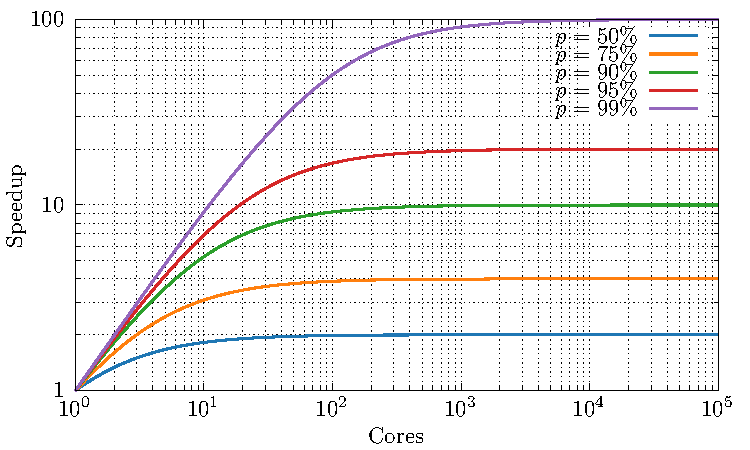
\includegraphics{assets/Amdahl/amdahl.pdf}
  \caption[Demonstration of Amhdal's law]{A demonstration of Amdahl's law, showing that as parallel fraction increases, there are significant gains in performance for a modest number of processing cores. Beyond a certain point, however, we find that speedup slows, and is asymptotic to a point where $S = 1/(1-p)$.}
  \label{fig:amdahl-demonstration}
\end{figure}

\begin{figure}
  \centering
  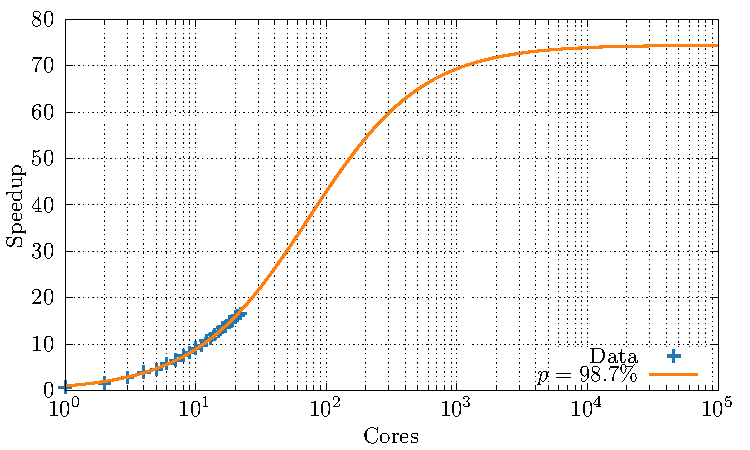
\includegraphics{assets/athena-amdahl/amdahl.pdf}
  \caption[Strong scaling test of \athena]{Strong scaling test of \athena{} running the simulation of WR140 as defined in chapter \ref{ch:wr140} for 100 timesteps. The parallel fraction of \athena{} running this problem is found to be 98.7\%. The test was conducted over 22 cores of a dual-processor \SI{2.1}{\giga\hertz} Intel Xeon Gold 6152 workstation using \texttt{hyperfine}. The second processor was not used as this introduced a penalty to performance due to inter-processor bandwidth bottlenecks.}
  \label{fig:amdahl-athena}
\end{figure}

Weak scaling is determined through Gustafson's law, which shows that as a problem increases in size to scale with the number of cores available, the theoretical speedup is linear

\begin{equation}
  S\rms{w}(N) = (1-p) + pN.
\end{equation}

\noindent
As $\lim_{N\rightarrow\infty} S_w = \infty$, there is no limit to the amount of scaling for an increasing problem size \parencite{gustafsonReevaluatingAmdahlLaw1988}.
As such we find that more powerful computers with many thousands of cores still benefit from parallelisation if the problem scales accordingly \parencite[Ch.~2]{pachecoIntroductionParallelProgramming2022}.

% Issues with parallelism at high amounts
Beyond these theoretical laws, there are practical limitations to parallel processing.
The first of which is die size and cost: a single large, multi-core processor would be extremely expensive to manufacture, while also reducing yield significantly due to manufacturing defects.
This was the basis of supercomputing, such as the vector processors manufactured by Cray, prior to the advent of Beowulf-based HPC clusters.
Intel attempted to solve this problem with KNL, implementing dozens of simple, slow cores and fast matrix math throughput, but these were impractical for a variety of reasons.
GPUs could also be considered an alternative implementation of this concept, and have seen much more success, chiplet-based designs such as AMDs Infinity Fabric or the Apple M1 Ultra.
Another issue is memory and communication bandwidth, as the problem scales to dozens of cores a single processing node would see reduced throughput due to memory bandwidth issues.
Furthermore as the problem scales beyond a single processor, we see a reduced level of performance as the programme has to leverage motherboard processor interconnects, or the much slower interconnects between nodes in an HPC cluster.

In testing \athena{} we found that the communication overhead became significant above 200 cores, with the current network topology and node availability of \texttt{ARC4}.
There was also an observed increase in communication overhead with \mg{} as well, as the programme handles parallelism by slicing the problem along the $y$ axis, resulting in a very large number of ``ghost'' cells that require communication.


\section{Datatypes \& visualisation}
\label{sec:visualisation}

Output data from \athena{} was exported at regular time-elapse intervals in the form of 3-D HDF5 files \parencite{hdf5} and 2-D slices at $z=0$ HDF5 files.
A separate, comma-delimited ``history'' filetype was written to regularly to store summated values of conserved variables and advected scalars.
This was used primarily to determine simulation-wide dust production rates and average grain sizes as the simulation evolved.
Checkpoint files were also written at regular intervals to ensure a restart in the event of a simulation crash or process kill by the ARC4 job-sharing queue system.
For most simulations 3-D data and checkpoints were saved every 1/\nth{100} of an orbital period, while 2-D data and ``history'' data was written every 1/\nth{1000} of an orbital period.

%//TODO section might not be necessary
Data was plotted using a series of custom programmes designed to parse data as quickly as possible, 
the \texttt{Python 3.8} \parencite{10.5555/1593511} plotting library provided in the \athena{} repository was modified to incorporate Delaunay triangulation, instead of interpolating static meshes to the finest level in order to operate correctly with \texttt{Matplotlib} \parencite{Hunter:2007}, data-points are triangulated with each other.
This is a markedly more memory and processing efficient method, as data is not duplicated or smoothed at the interpolation step, and was found to be approximately 2000\% faster.
Whilst this can result in artefacts at low resolutions, the resolution of the simulation was sufficient such that these artefacts were not observed.
The GNU Parallel library was used to batch-process 2D exports \parencite{tange_2021_5523272}, as \texttt{Python} is for the most part single threaded and interpreted it was found to be more effective use Parallel to run multiple python instances at once, each processing a single data file using the command:

\begin{lstlisting}[language=bash]
seq 0 <max> | parallel -j44  "athena_plot.py plot-config.yaml -n {}"
\end{lstlisting}

\noindent
where \texttt{<max>} is the number of simulation files.
The \texttt{Numba} library \parencite{lam2015numba} was also used to improve performance by  JIT\footnote{Just In Time.} compiling, parallelising and vectorising certain steps that were not performant in either \texttt{Python} or \texttt{Numpy} \parencite{harris2020array}.
In this case, \texttt{Numba} was used to restructure numerical array data into a linear series of arrays, performing derived parameter such as dust density and temperature calculations, and matrix co-ordinate transforms.
While this is less straightforward to implement, as many of \texttt{Pythons} data-types cannot be used, this offered a 2 order of magnitude processing speed increase in the case of an 8-core workstation.

For 3D visualisation the \texttt{VisIt} application is used \parencite{HPV:VisIt}.
However for print 2D slices generated using \texttt{Matplotlib} were used. 
The \texttt{Gnuplot} utility \parencite{gnuplot} was used for generating line and scatter plots throughout this thesis, in particular history outputs from \athena{}.
Occasionally, rendering video of the batch processes 2D exports was performed in order to better understand how the systems propagated over time, in order to do this \texttt{ffmpeg} library \parencite{tomar2006converting} was used to render the videos.
For this, the following command was used:

\begin{lstlisting}[language=bash]
cat /*.png | ffmpeg -f image2pipe -framerate 30 -i - -c:v libx264 -vf format=yuv420p output.mp4
\end{lstlisting}

\section{Version Control}

This is going to be a very short section, as it is more of a plea to other doctoral students who read this - especially those starting out.
Use version control in your projects, the number of times I lost work or code because I did not use version control software like \texttt{Git} in my first year is frankly far too high.
It'll save you a lot of time in the long run, trust me.

\noindent
Keep your thesis on there too.